% !TEX root = lac.tex
\section{Introduction}
\label{intro}

Due to the recent developments of gigantic social networks (e.g., Flickr, Facebook, and Twitter), the topic of {\it attributed graphs} has attracted attention from industry and research communities~\cite{attr-topic-sigmod2012,keyword-icde2002,keyword-icde2007,keyword-sigmod2007,keyword-vldb2005,keyword-yu-2009,keyword-vldb2011,fang2014}.  An attributed graph is essentially a graph associated with text strings or keywords.  Figure~\ref{fig:motivation} illustrates an attributed graph, where each vertex represents a social network user, and its keywords describe the interest of that user.

\begin{figure}
	\small
	\centering
	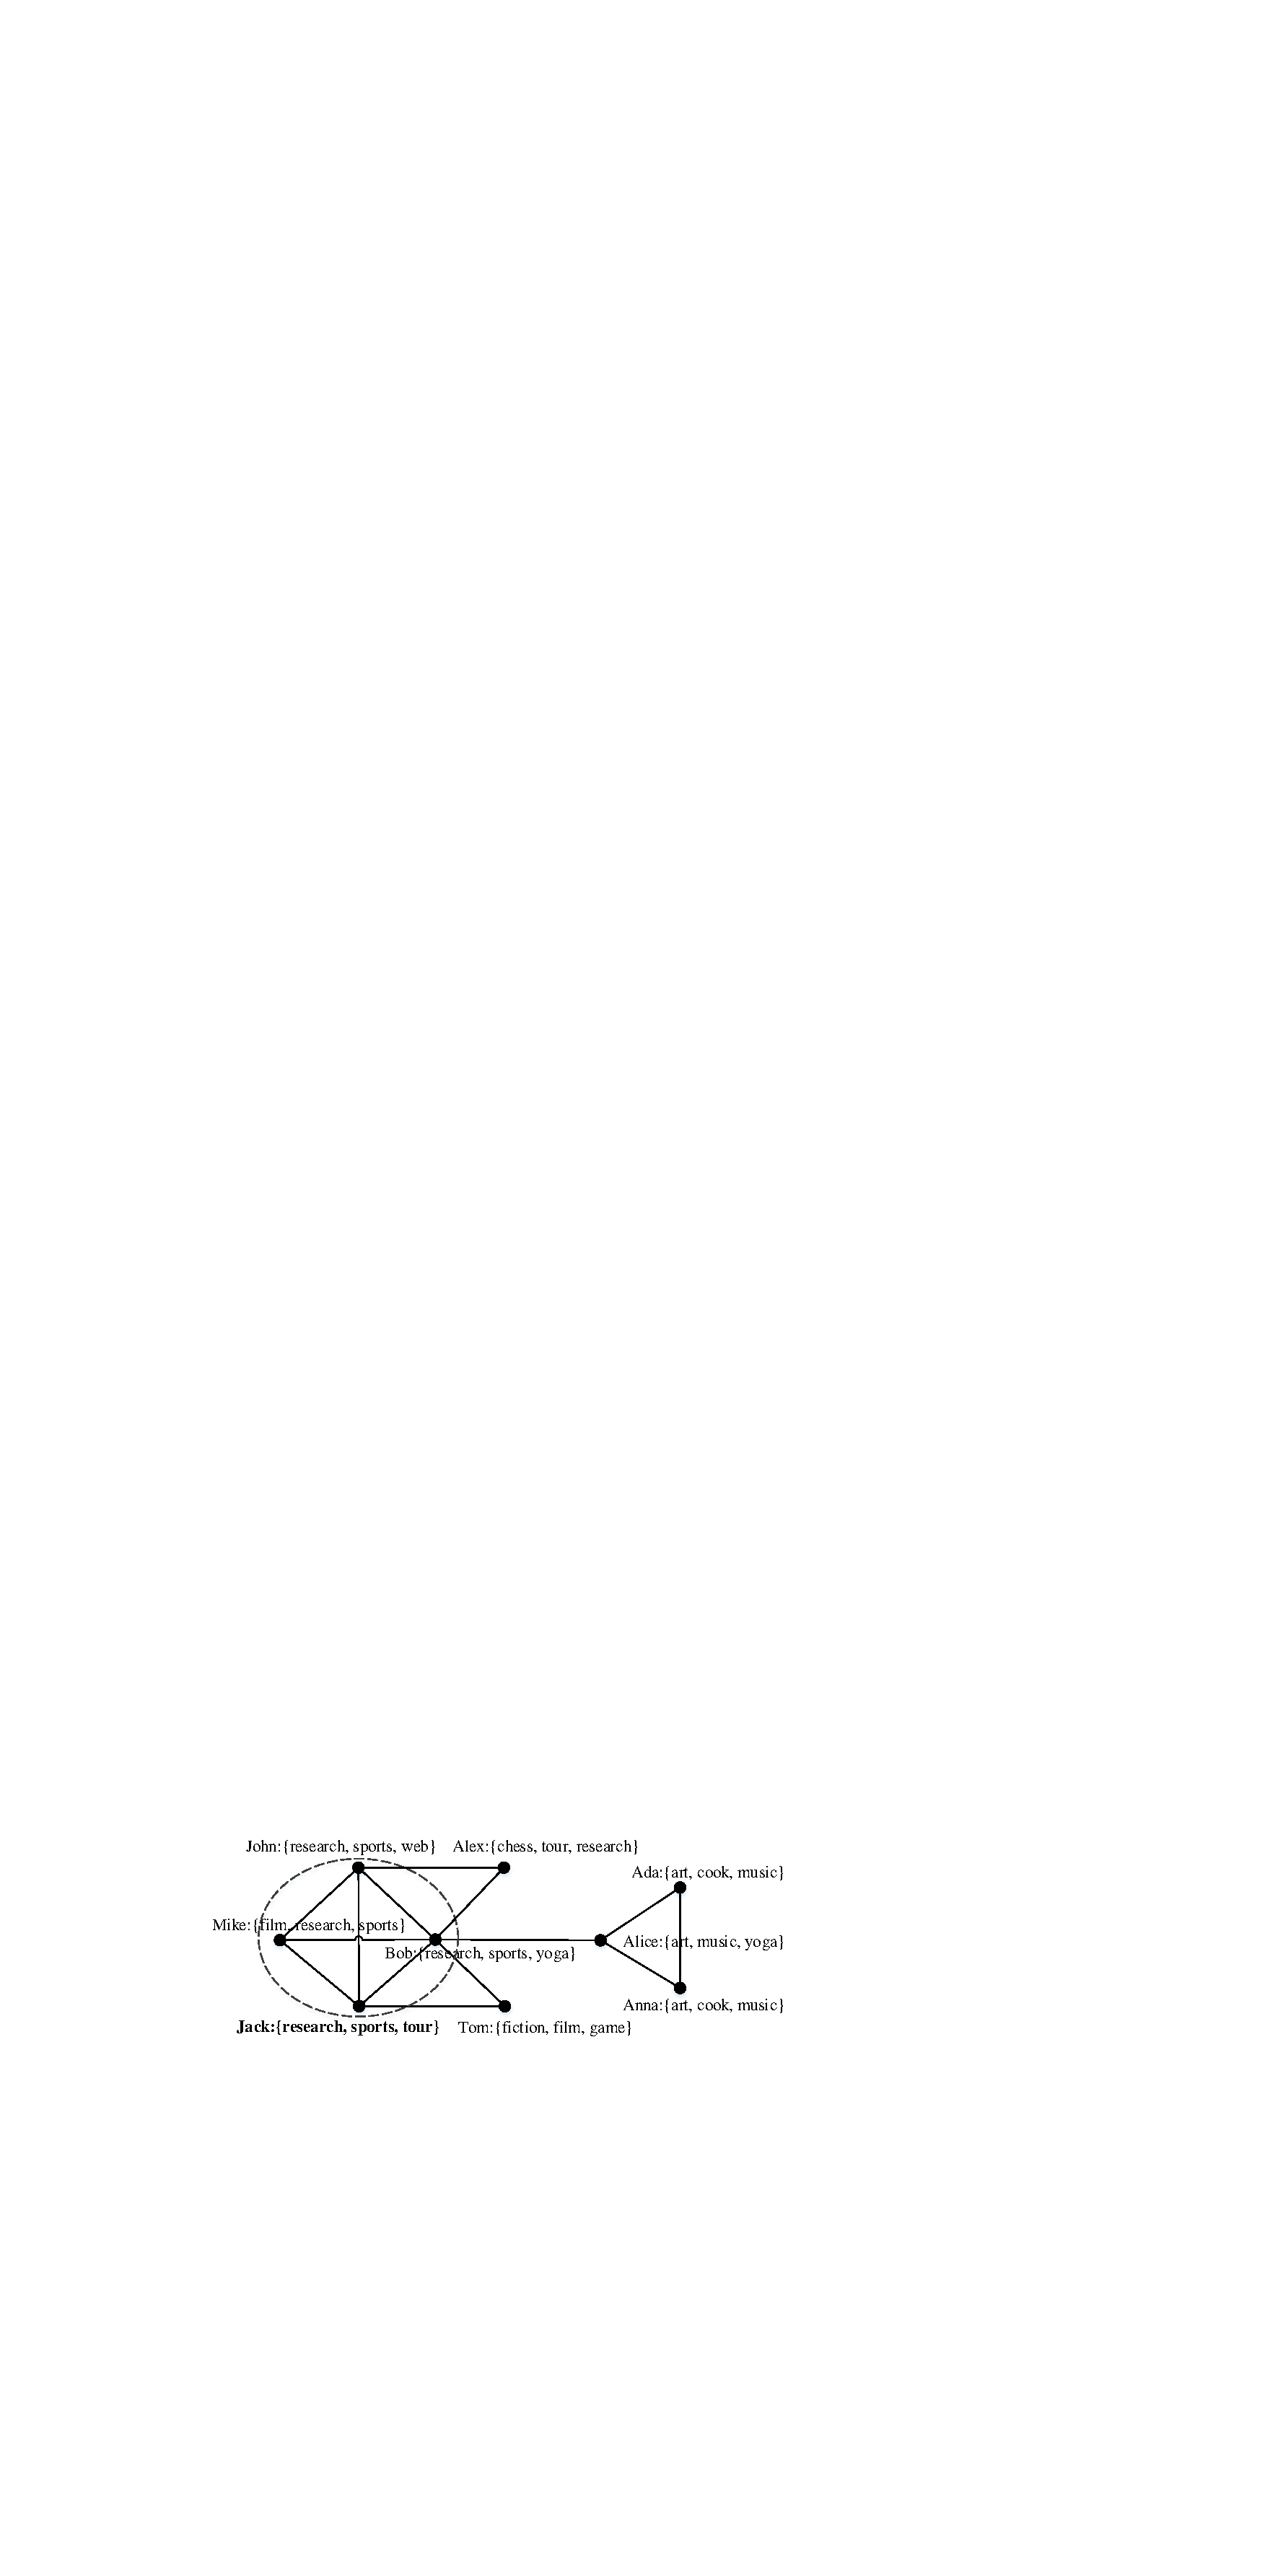
\includegraphics[width=0.88\linewidth]{figures/motivation}
	\caption{Attributed graph and AC (circled).}
	\label{fig:motivation}
\end{figure}

In this paper, we investigate the {\it attributed community query} (or ACQ). Given an attributed graph $G$ and a vertex $q \in G$, the ACQ returns one or more subgraphs of $G$ known as {\it attributed communities} (or ACs).  An AC is a kind of {\it community}, which consists of vertices that are closely related~\cite{KDD2010,local2014,online-sigmod2013,k-truss2014,community-phy2004,community-phy2010}.  Particularly, an AC satisfies {\it structure cohesiveness} (i.e., its vertices are closely linked to each other) and {\it keyword cohesiveness} (i.e., its vertices have keywords in common). Figure~\ref{fig:motivation} illustrates an AC (circled), which is a connected subgraph with vertex degree 3; its vertices $\{${\tt Jack}, {\tt Bob}, {\tt John}, {\tt Mike}$\}$ have two keywords (i.e., ``research'' and ``sports'') in common.

{\bf Prior works.} %An AC is a kind of {\it community}.
The problems related to retrieving communities from a graph can generally be classified into {\it community detection} (CD) and {\it community search} (CS).  In general, CD algorithms aim to retrieve all communities for a graph~\cite{community-phy2004,community-phy2010,attr-vldb2009,attr-topic-kdd2008,attr-topic-icml2009,attr-topic-sigmod2012,attr-www2013,yang2013community}. These solutions are not ``query-based'', i.e., they are not customized for a query request (e.g., a user-specified query vertex).
%For example, it is not clear how these algorithms can return a community that contain a given vertex $q$.
Moreover, they can take a long time to find all the communities for a large graph, and so they are not suitable for quick or {\it online} retrieval of communities. To solve these problems, CS solutions have been recently developed~\cite{KDD2010,local2014,online-sigmod2013,k-truss2014,huang2015approximate,barbieri2015efficient}. These approaches are query-based, and are able to derive communities in an ``online'' manner. However, existing CS algorithms assume {\it non-attributed} graphs, and only use the graph structure information to find communities. The ACQ is a class of CS problem for attributed graphs. As we will show, the use of keyword information can significantly improve the effectiveness of the communities retrieved. Table~\ref{tab:method} summarizes some representative existing works in this area.

\begin{table}
  \centering \footnotesize \caption {Classification of works in community retrieval. }\label{tab:method}
  \begin{tabular}{c|c|c}
     \hline
        \tabincell{c}{\textbf{Graph}\\ \textbf{Type}}
                       & \tabincell{c}{\textbf{Community}\\ \textbf{detection (CD)}}
                       & \tabincell{c}{\textbf{Community}\\ \textbf{search (CS)}}\\
     \hline\hline
        Non-attributed & \cite{community-phy2004,community-phy2010}
                       & \cite{KDD2010,local2014,online-sigmod2013,k-truss2014,vldb2015,huang2015approximate}\\
     \hline
        Attributed     & \cite{attr-vldb2009,attr-topic-kdd2008,attr-topic-icml2009,attr-topic-sigmod2012,attr-www2013,yang2013community}
                       & {\bf ACQ}\\
     \hline
  \end{tabular}
\end{table}

{\bf Features of ACs.} We now present more details about ACs.

\noindent $\bullet$ {\bf Ease of interpretation.}
As demonstrated in Figure~\ref{fig:motivation}, an AC contains tightly-connected vertices with similar contexts or backgrounds. Thus, an ACQ user can focus on the common keywords or features of these vertices (e.g., the vertices of the AC in this example contain ``research'' and ``sports'', reflecting that all members of this AC like research and sports).  We call the set of common keywords among AC vertices
the \emph{AC-label}. In our experiments, the AC-labels facilitate understanding of the vertices that form the AC.

The design of ACs allows it to be used in setting up of social events. For example, if a Twitter member has many keywords about traveling (e.g., he posted a lot of photos about his trips, with keywords), issuing an ACQ with this member as the query vertex may return other members interested in traveling,  because their vertices also have keywords related to traveling. A group tour can then be recommended to these members.

\noindent $\bullet$ {\bf Personalization.}  The user of an ACQ can control the semantics of the AC, by specifying a set of $S$ of keywords. Intuitively, $S$ decides the meaning of the AC based on the user's need.  If we let $q$={\tt Jack}, $k$=2 and $S$=$\{$``research''$\}$,  the AC is formed by
$\{${\tt Jack}, {\tt Bob}, {\tt John}, {\tt Mike}, {\tt Alex}$\}$, who are all interested in research.
Let us consider another example in the DBLP bibliographical network, where each vertex's attribute is represented by the top-20 frequent keywords in their publications. Let $q$={\tt Jim} {\tt Gray}. If $S$ is the set of keywords \{transaction, data, management, system, research\}, we obtain the AC in Figure~\ref{fig:jim}(a), which contains six prominent database researchers closely related to Jim. On the other hand, when $S$ is \{sloan, digital, sky, survey, SDSS\}, the ACQ yields another AC in Figure~\ref{fig:jim}(b), which indicates the seven scientists involved in the SDSS project~\footnote{URL of the SDSS project: \url{http://www.sdss.org}.}.  Thus, with the use of different keyword sets $S$, different ``personalized'' communities can be obtained.

Existing CS algorithms, which do not handle attributed graphs, may not produce the two ACs above. For example, the CS algorithm in \cite{KDD2010} returns the community with {\it all} the 14 vertices shown in Figures~\ref{fig:jim}(a) and (b). The main reasons are: (1) these vertices are heavily linked with Jim; and (2) the keywords are not considered. In contrast, the use of set $S$ in the ACQ places these vertices into two communities, containing vertices that are cohesive in terms of {\it structure} and {\it keyword}. This allows a user to focus on the important vertices that are related to $S$. For example, using the AC of Figure~\ref{fig:jim}(a), a database conference organizer can invite speakers who have a close relationship with Jim.

The personalization feature is also useful in marketing. Suppose that Mary, a yoga lover, is a customer of a gym. An ACQ can be issued on a social network, with Mary as the query vertex and $S$=$\{$``yoga''$\}$. Since members of the AC contain the keyword ``yoga'', they can be the gym's advertising targets. On the other hand, current CS algorithms may return a community that contains one or more vertices without the keyword ``yoga''. It is not clear whether the corresponding user of this vertex is interested in yoga.

\noindent $\bullet$ {\bf Online evaluation.}  Similar to other CS solutions, we have developed efficient ACQ algorithms for large graphs, allowing ACs to be generated quickly upon a query request. On the contrary, existing CD algorithms~\cite{attr-vldb2009,attr-www2013,attr-topic-kdd2008,attr-topic-icml2009} that generate all communities for a graph are often considered to be offline solutions, since they are often costly and time-consuming, especially on very large graphs.

{\bf Technical challenges and our contributions.}
We face two important questions: (1) What should be a sound definition of an AC? (2) How to evaluate ACQ efficiently?  For the first question, we define an AC based on the {\it minimum degree}, which is one of the most common structure cohesiveness metrics~\cite{community-phy2004,community-phy2010,KDD2010,local2014}. This measure requires that every vertex in the community has a degree of $k$ or more.
%one of the most fundamental characteristics of graphs, and some recent works~\cite{KDD2010,local2014} have shown that it is better than many other metrics like average degree and density of a graph.
We formulate the keyword cohesiveness as maximizing the number of shared keywords in keyword set $S$. The shared keywords naturally reveal the common features among vertices (e.g., common interest of social network users). We can also use these shared keywords to explain how a community is formed.

\begin{figure}[ht]
    \centering
    \mbox{
        \subfigure[$S$=\{transaction, data, management, system, research\}]{
            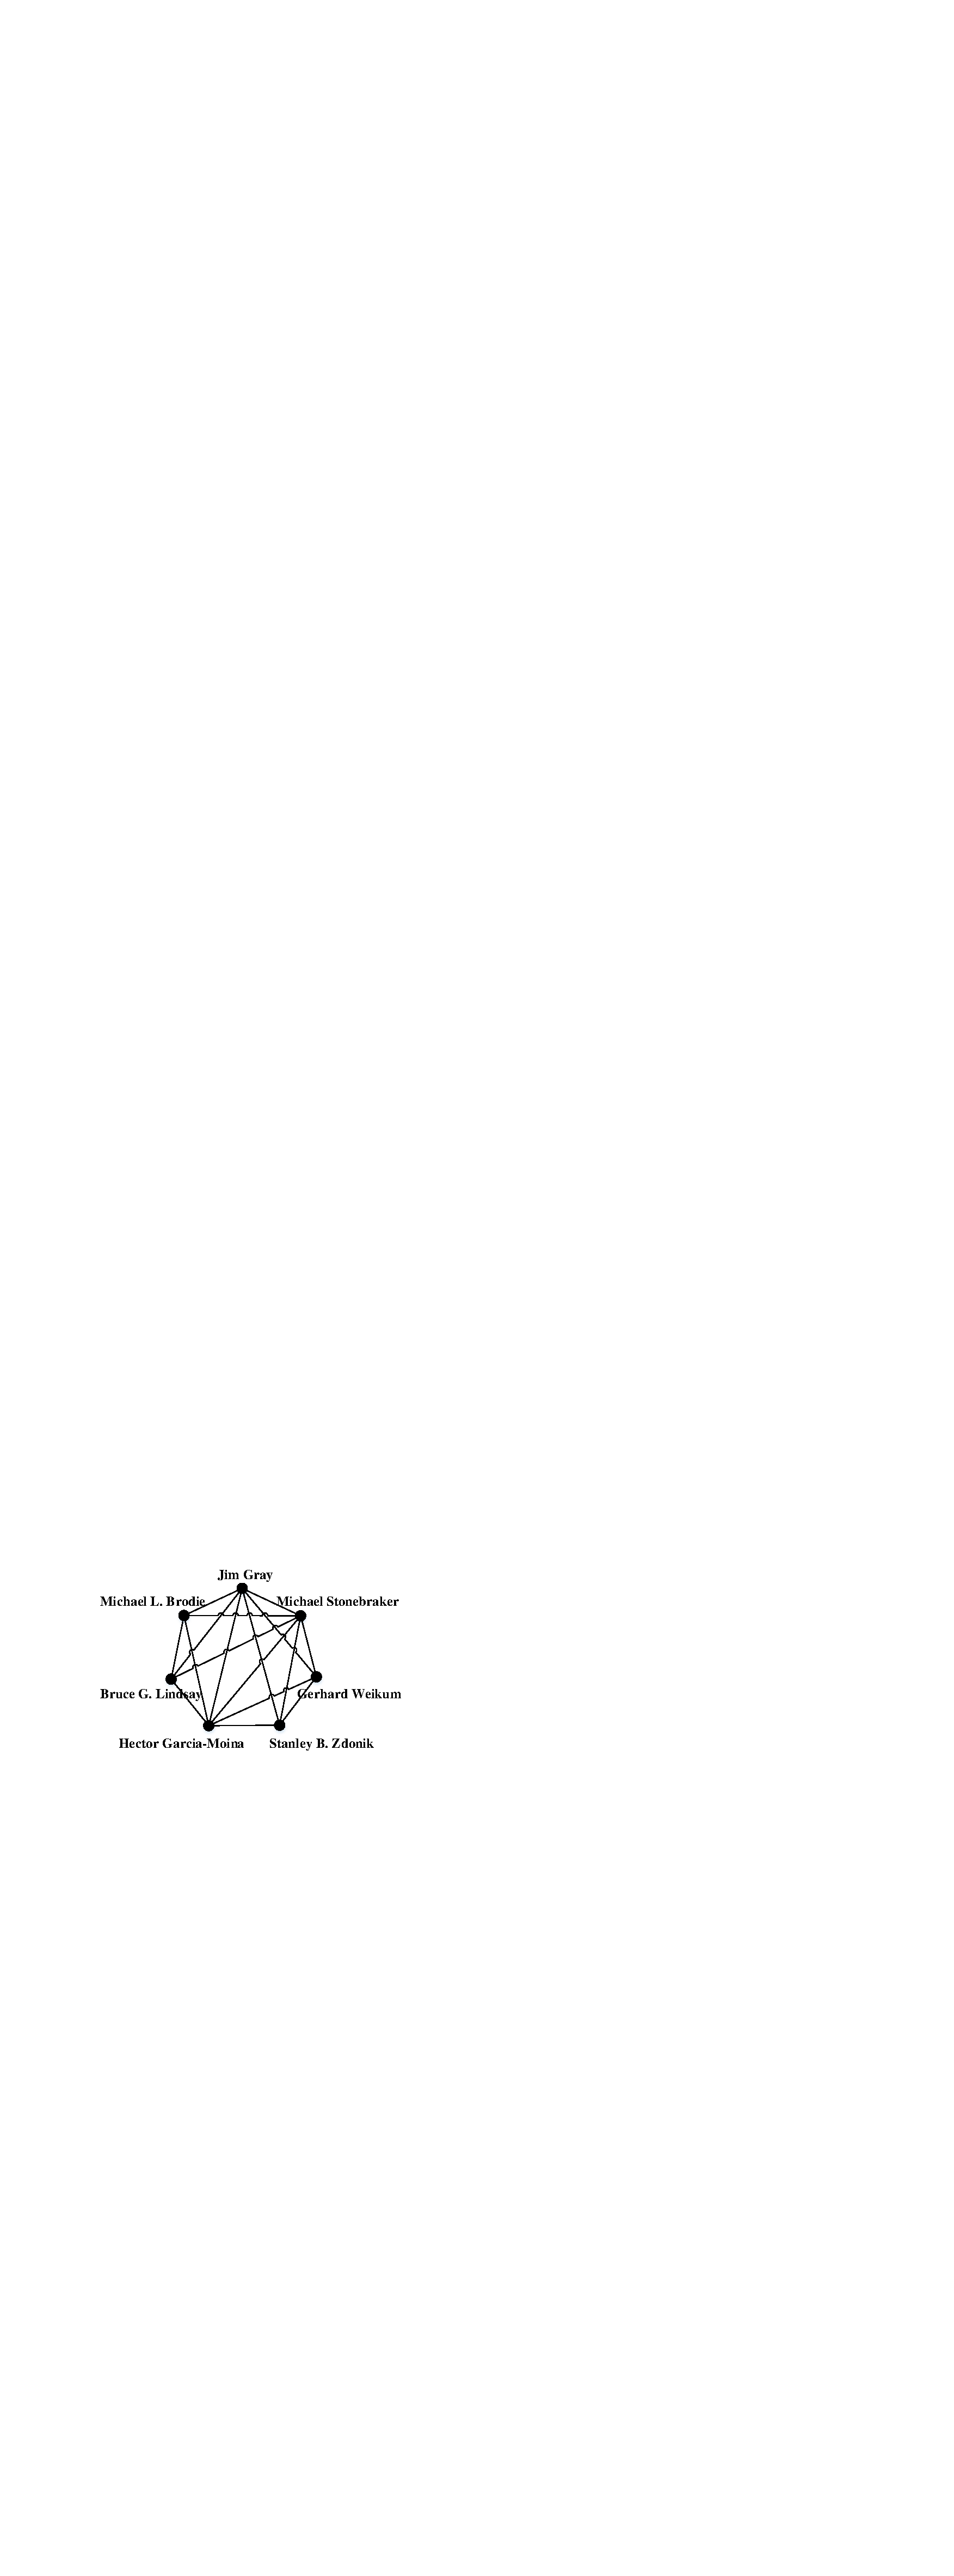
\includegraphics[width=.44\columnwidth]{figures/jim1}
            \label{fig:jim1}
        }
        \hspace{1ex}
        \subfigure[$S$=\{sloan, digital, sky, data, sdss\}]{
            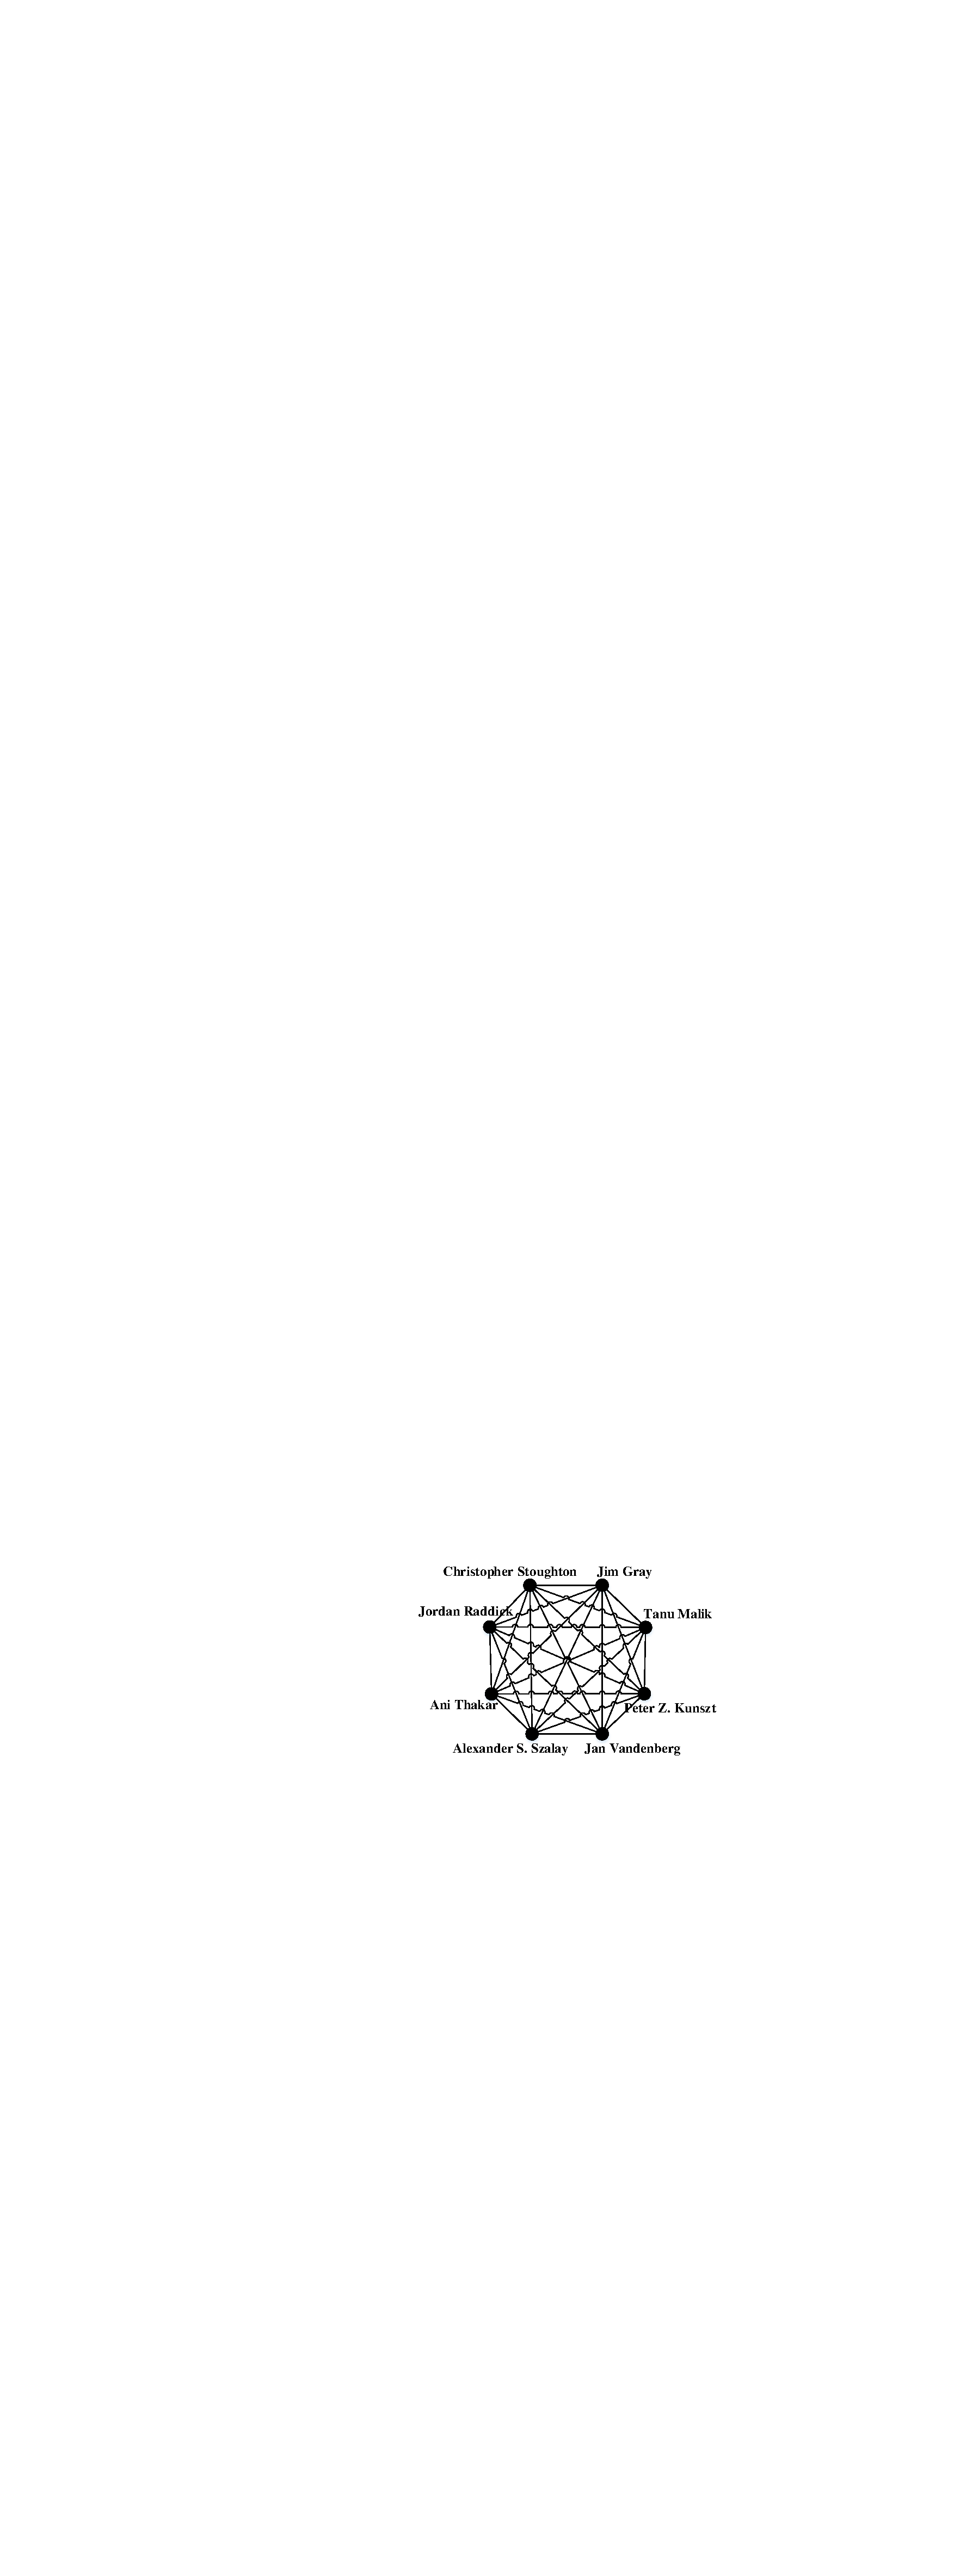
\includegraphics[width=.432\columnwidth]{figures/jim2}
            \label{fig:jim2}
        }
    }
    \caption{Two ACs of Jim Gray.}\label{fig:jim}
\end{figure}

The second question is not easy to answer, because the attributed graph $G$ to be explored can be very large, and the (structure and keyword) cohesiveness criteria can be complex to handle. A simple way is first to consider all the possible keyword combinations, and then return the subgraphs, which satisfy the minimum degree constraint and have the most shared keywords. This solution, which requires the enumeration of all the subsets of $q$'s keyword set, has a complexity exponential to the size $l$ of $q$'s keyword set. In our experiments, for some queries, $l$ can be up to 30, resulting in the consideration of $2^{30}=1,073,741,824$ subsets of $q$. The algorithm is impractical, especially when $q$'s keyword set is large.

{\color{blue}
We observe the {\it anti-monotonicity} property, which states that given a set $S$ of keywords, if it appears in every vertex of an AC, then for every subset $S'$ of $S$, there exists an AC in which every vertex contains $S'$. We use this intuition to propose better algorithms. We further develop the \emph{CL-tree}, an index that organizes the vertex keyword data in a hierarchical structure. The CL-tree has a space and construction time complexity linear to the size of $G$.
Based on the CL-tree index, we have developed three different ACQ algorithms, and they are able to achieve a superior performance.
In practice, graphs are continuously evolving \cite{chenghui,kddEvolving}. For instance, in the friendship networks of Facebook, users may change their profiles, and make new friends or remove friendship. Thus the CL-tree index needs to be updated to reflect the changes in the graph. A straightforward method to handle the update is to rebuild the CL-tree from scratch. However, this can be very computationally expensive, especially when the updates are very frequent. To alleviate this issue, we have developed efficient algorithms to maintain the CL-tree index for dynamic graphs.

In addition, we have proposed two typical variants of the ACQ problem, which are called {\it Approximate ACQ problem} (or ACQ-A) and {\it Multiple-vertex ACQ problem} (or ACQ-M) respectively.
ACQ-A is an approximation version of the ACQ query, in which vertices of an AC do not need to exactly share the same keywords as that in ACQ. It relaxes the constraint on sharing common keywords; this could be very useful if the vertices of the graph do have much keyword information.
ACQ-M generalizes the ACQ query for supporting multiple query vertices. It takes multiple query vertices as input and returns the ACs containing all of them. This could be very useful if we want to find the ACs for a group of query vertices. For example, a database workshop organizer may be interested in inviting researchers who have a close relationship with both Jim Gray and Michael Stonebraker.
To answer the queries for ACQ-A and ACQ-M, we have also developed efficient algorithms based on the CL-tree index.
}

We have performed extensive experiments on six large real graph datasets.
We found that a large number of common keywords appear across vertices in our graph datasets. In DBLP, for instance, an AC with one common keyword contains over 5,000 vertices on average; an AC with two common keywords contains over 700 vertices. Hence, using shared keywords among vertices as keyword cohesiveness makes sense.
We have also studied how to quantify the quality of a community, based on occurrence frequencies of keywords and similarity between the keyword sets of two vertices. We conducted a detailed case study on DBLP. These results confirm the superiority of the AC over the communities returned by existing community detection and community search algorithms, in terms of community quality. The performance of our best algorithm is 2 to 3 order-of-magnitude faster than solutions that do not use the CL-tree. 
We have also experimentally evaluated the index maintenance algorithms and the results show that they are very efficient.
Moreover, we perform the queries of the ACQ-A and ACQ-M problems, and the results show that our index-based algorithms are much faster than the baseline algorithms. In addition, our approaches achieve a higher efficiency than existing community search solutions (that do not use vertex keywords in the community search process).

{\bf Organization.} We review the related work in Section~\ref{related}, and define the ACQ problem formally in Section~\ref{problem}. Section~\ref{basic} presents the basic solutions, and Section~\ref{index} discusses the CL-tree index.
In Section~\ref{indexMaintenance}, we discuss how to maintain the CL-tree index for dynamic graphs.
We present the query algorithms in Section~\ref{query}.
In Section~\ref{variant}, we introduce two variants and the corresponding query algorithms.
Our experimental results are reported in Section~\ref{experiment}.
We conclude in Section~\ref{conclusion}. 